\research{WORKSHEET 10 Computer Structure and Function}{27-01-23}{Worksheet}

\begin{enumerate}
    \item \textbf{What is Computer Architecture? What is Computer Organisation? What are the main differences between them, explain them using examples?}\\
    Computer architecture is the attributes of the computer that have a direct impact on the logical execution of a program (for example there will need to be some form of memory and some form of addition unit). Computer organisation is the operational units and their interconnections (for example the vacuum tubes or transistors).
    \item \textbf{What are the four main functions of a computer?}\\
    Data processing, data storage, data movement, control.
    \item \textbf{Explain the functional view of a computer with the help of a flow chart.}
    \begin{figure}[H]
        \centering
        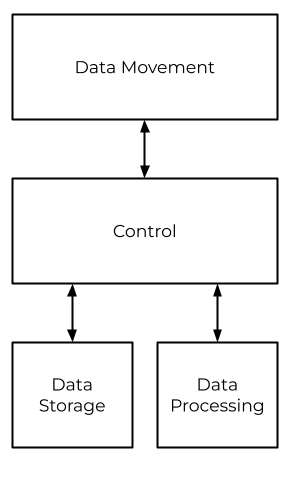
\includegraphics[width=0.3\textwidth]{assets/functional-view-computer.png}
        \caption{Functional view of a computer}
    \end{figure}
    In the above diagram, the arrows represent the movement of data throughout the blocks. The data moves from the `movement block' where it interfaces with external peripherals. The data moves through the `control block' where it can either go to the `data storage' or `data processing' blocks.
    \item \textbf{Explain with a simple diagram the internal structure of the computer.}
    The diagram below shows the internal structure of a computer. The main memory, input and output devices, and CPU are connected together by the `system bus'. Through this, they can share data between them.
    \begin{figure}[H]
        \centering
        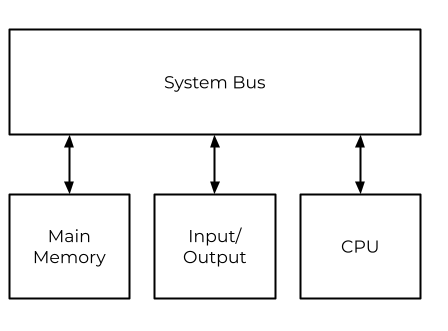
\includegraphics[width=0.4\textwidth]{assets/computer-internal-structure.png}
        \caption{Internal structure of a computer}
    \end{figure}
    \item \textbf{List and define the main structural components of a processor.}\\
    The CPU has a number of components within it.

    The \textit{Arithmetic \& Logic Unit (ALU)} is an adder/ subtractor and performs the arithmetic and logical operations which we learnt about in Teaching Block 1.

    The \textit{Registers} are very small amounts of extremely fast memory. Register memory is very expensive. Registers are used to hold the data which is going to/ from main memory.

    The \textit{Internal Bus} is the internal communications line within the CPU.

    The \textit{Control Unit (CU)} is the `heart' of the CPU. It signals to other components of the CPU to keep them in sync. The CU contains sequencing logic, CU registers and decoders, and control memory; these are beyond the scope of this course.

    \item \textbf{What was the main technology used in the first generation of computers? Describe its technology.}\\
    The first generation of computers used vacuum tubes. Vacuum tubes work by heating up a filament which releases electrons (negatively charged). These move towards the positively charged plate (anode) which causes a current to flow.

    \item \textbf{What is ENIAC and explain its working process(e.g. accumulators)?}\\
    ENIAC was manually programmed and worked using decimal, not binary.

    \item \textbf{What is a stored-program concept?}\\
    The stored program concept is where the program contents is stored in main memory then during run-time it is fetched, executed and decoded.

    \item \textbf{Explain with a simple diagram the von Neumann machine architecture.}
    \begin{figure}[H]
        \centering
        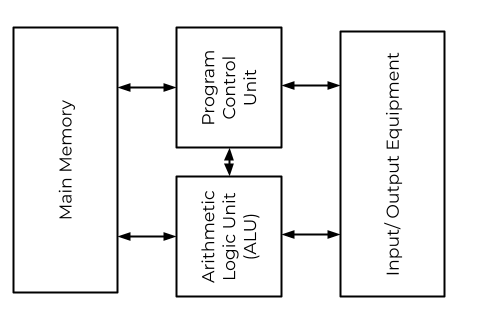
\includegraphics[width=0.5\textwidth]{assets/von-neumann-architecture.png}
        \caption{Von Neumann architecture}
    \end{figure}

    \item \textbf{What is the difference between ALU and control units?}\\
    The ALU (Arithmetic Logic Unit) is where the arithmetic and logical operations are performed whereas the Control Unit is the part of the CPU which synchronises all the other operations within the CPU.

    \item \textbf{Explain IAS memory structure.}\\
    Memory has 1000 locations, each 1 word (40 bits) long. Could either store one number (where MSB is sign bit) or two instructions (each 20 bits long).

    \item \textbf{What are the differences between Number and Instruction words in IAS computers?}\\
    Number words are 40 bits long (1 word) however instructions are 20 bits long (1/2 word). This means two instructions can fit into one word.

    \item \textbf{Why are two different kinds of words used in von Neumann architecture?}\\
    We need to store instructions and numbers in the same memory.

    \item \textbf{What are Opcodes and addresses in instruction words?}\\
    Opcodes (8-bits) are the operation which is to be performed; for example, add, subtract. Addresses (12-bits) is the address which the opcode is to be performed on.
    
    \item \textbf{What are the advantages and disadvantages of von Neumann architecture?}\\
    As there is a shared instructions and data memory, you can only access one or the other at once which decreases performance. As the memory is shared, both the instructions and data have to be the same size. 
\end{enumerate}